\documentclass[../../main.tex]{subfiles}

\begin{document}

\chapter{Foundations}

Before getting into different techniques and methods, let's discuss
fundamental topics including time complexity and basic DSA.

\section{Time Complexity}

One of the primary goal of competitive programming and an effective
program is efficiency. Indeed most, if not all, programming
competitions have time limits, which varies for each language.
Some problems can be solved with brute force approach while others
need an elegant solution to fit in the given time frame.

\begin{definition}{}{}
The \textbf{Time Complexity} of a program denotes the number of
operations an algorithm executes \cite{CS02-5}.
\end{definition}

Please note that the definition above is very basic, and not formal.
A more formal definition involves theoretical computer science, and
maybe I can include more on the formal definition and P = NP in
other notes.

The approximate number of the operations for the worst-case is
represented using the \textbf{big O notation}. The lower the
complexity, the efficient the program is.

The six major complexities are Constant $\mathcal{O}(1)$, Linear
$\mathcal{O}(n)$, Logarithmic $\mathcal{O}(n \log n)$, Quadratic
$\mathcal{O}(n^2)$, Exponential $\mathcal{O}(2^n)$, and Factorial
$\mathcal{O}(n!)$ \cite{CS02-8}. We will evaluate the time
complexities of algorithms as we walk through them, but here are
some simple examples using input/output and loops.

A simple hello world example have constant time complexity since it
only prints once. One the other hand, the following snippet

\begin{basicbox}
\begin{lstlisting}[style=cppstyle]
for (int i = 0; i < 5*n; i++) {
    // constant time code
}
\end{lstlisting}
\end{basicbox}

is $\mathcal{O}(n)$ \cite{CS02-2}. When we start nesting them,
it gets horrible. For instance, the following snippet is
$\mathcal{O}(nm)$.

\begin{basicbox}
\begin{lstlisting}[style=cppstyle]
for (int i = 0; i < n; i++) {
    for (int j = 0; i < m; j++) {
        // constant time code
    }
}
\end{lstlisting}
\end{basicbox}

Naturally, we can see that we get quadratic time if we nest code
as the following.

\begin{basicbox}
\begin{lstlisting}[style=cppstyle]
for (int i = 0; i < n; i++) {
    for (int j = 0; i < n; j++) {
        // constant time code
    }
}
for (int i = 0; i < 10000*n; i++) {
    // constant time code
}
\end{lstlisting}
\end{basicbox}

The snippet above is $\mathcal{O}(nn) = \mathcal{O}(n^2)$. Note that
the time complexity is not linear since the big O is only interested
in the worst case.

One more thing to note is the order of growth. Consider the graph
below \cite{CS02-8}.

\begin{figure}[H]
\centering
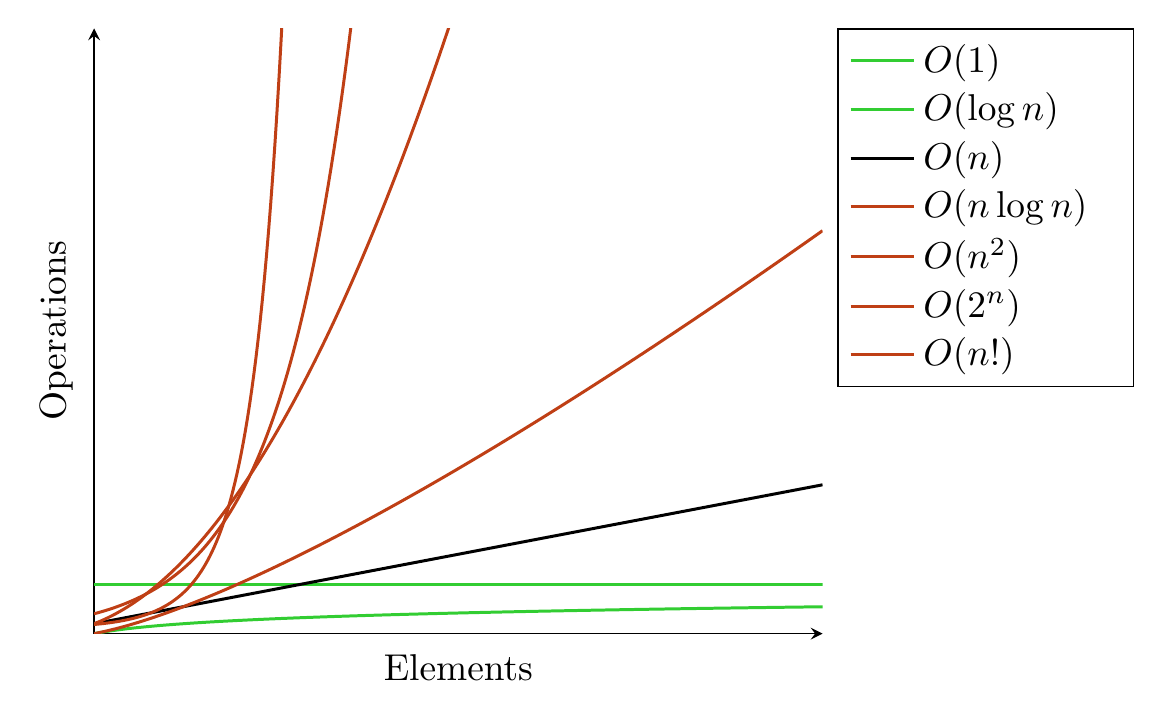
\begin{tikzpicture}[scale=1.35]
\begin{axis}[
    axis lines=left,
    xlabel={Elements},
    ylabel={Operations},
    xmin=1, xmax=15,
    ymin=0, ymax=61,
    domain=1:15,
    samples=200,
    legend style={
        at={(1.02,1)},
        anchor=north west,
        align=left,
        text width=1.8cm
    },
    xtick=\empty, ytick=\empty
]

\addplot[
    LimeGreen, thick,
    domain=1:15,
    samples=100
]{5};
\addlegendentry{$O(1)$}

\addplot[
    LimeGreen, thick,
    domain=1:15,
    samples=100
]{ln(x)};
\addlegendentry{$O(\log n)$}

\addplot[
    black, thick,
    domain=1:15,
    samples=100
]{x};
\addlegendentry{$O(n)$}

\addplot[
    Bittersweet, thick,
    domain=1:15,
    samples=100
]{x*ln(x)};
\addlegendentry{$O(n \log{n})$}

\addplot[
    Bittersweet, thick,
    domain=1:8,
    samples=100
]{x^2};
\addlegendentry{$O(n^2)$}

\addplot[
    Bittersweet, thick,
    domain=1:6.5,
    samples=100
]{2^x};
\addlegendentry{$O(2^n)$}

\addplot[
    Bittersweet, thick,
    domain=1:5,
    samples=100
]{sqrt(2*pi*x)*(x/e)^x};
\addlegendentry{$O(n!)$}
\end{axis}
\end{tikzpicture}
\end{figure}

From the graph above, we can see that some functions grow faster
than the other. For instance, the constant time has the lowest
growth rate since it is not growing at all. Next, we can see
that $\log{n}$ grows slower than $n$, which grows slower than
$n \log{n}$ \cite{CS02-5}. Generally speaking, anything below
$\mathcal(n)$ is good while we really want to avoid anything
beyond the linear time.

Now big O is important since it is used to compare two algorithms
that perform the same task. With \textbf{asymptotic analysis},
we can evaluate and compare algorithms without the inconsistency
of inputs and machines \cite{CS02-5}. This was a short introduction
to computing time complexities and big O notation. In the next
section, we will be discussing fundamental data structures.

\end{document}


